\documentclass[a4paper, 12pt]{article}

\usepackage[utf8]{inputenc}
\usepackage[T1]{fontenc}
\usepackage{graphicx}
\usepackage[portuguese]{babel}
\usepackage[top=2cm,right=2cm,bottom=2cm,left=2cm]{geometry}
\usepackage{hyperref}
\usepackage{fontspec}
\setmainfont{Arial}
\usepackage{xwatermark}
\usepackage{xcolor}
\newwatermark[allpages, scale=7, angle=60, color=gray!10, xpos=-20, ypos=20]{FA503}

\newcommand{\qs}[1]{\noindent\textbf{Questão #1}}

\begin{document}
	\begin{flushleft}
		\textbf{Nome:} Renan da Silva Guedes\\
		\textbf{RA:} 223979
	\end{flushleft}
		

		\qs{1}
		
		\hspace{.2cm}Tempo é o conjunto das condições atmosféricas de determinado lugar em determinado momento. Clima é a média das condições atmosféricas desse lugar; ou seja, é o resultado da repetição de um determinado tipo de tempo nesse lugar por anos sucessivos.\\
		
		\qs{2}
	
		\hspace{.2cm}Representa os eventos que compõem o tempo atmosférico responsáveis pela caracterização do clima.\\
		
		\qs{3}
			
		\hspace{.2cm}Fatores são agentes causais que
		condicionam os elementos meteorológicos, associados aos aspectos físicos.
		
		\begin{itemize}
			\item\href{http://www.leb.esalq.usp.br/leb/aulas/lce306/Aula2_2012.pdf}{Link (ESALQ/USP)}
		\end{itemize}
		
		\qs{4}
		
		\hspace{.2cm}A radiação solar pode ser tomada
		tanto como elemento, por ser uma variável
		que quantifica a disponibilidade de energia
		solar na superfície terrestre, como também
		pode ser considerada um fator, por
		condicionar a temperatura, a pressão e
		indiretamente outros elementos meteorológicos
		
		\begin{itemize}
			\item\href{http://www.leb.esalq.usp.br/leb/aulas/lce306/Aula2_2012.pdf}{Link (ESALQ/USP)}
		\end{itemize}
		
		\qs{5}
		
		\hspace{.2cm}As estações do ano são estabelecidas com base na posição relativa Terra - Sol tomando-se o equador terrestre como referencial. No decorrer do tempo a Terra ao descrever um movimento de rotação e translação causa variação no ângulo de declinação solar ($\delta$). Por percorrer uma trajetória elíptica as regiões da Terra recebem diferentes níveis de luz incidente em sua superfície e isso torna o movimento aparente do Sol distinto ao longo do tempo. Dessa forma, é possível ter maior incidência de luz em um dos hemisférios, caracterizando os solstícios ou de forma igualmente distribuída na linha do Equador, o que caracteriza o equinócio. Logo, as diferentes taxas de energia absorvidas pelas regiões da Terra promovem a variação do gradiente de temperatura na sua superfície.
		
		\begin{itemize}
			\item\href{http://www.observatorio.ufmg.br/pas44.htm}{Link (Observatório UFMG)}
		\end{itemize}
		
		\qs{6}
		
		\hspace{.2cm}Os verões são caracterizados por elevadas temperaturas acompanhadas de altos índices pluviométricos. Nesse período, por estar no solstício de verão os dias são mais duradouros e a incidência solar aproxima-se da normal a superfície terrestre. No outono ocorre queda gradativa das temperaturas, exceto nas regiões próximas à linha do Equador. O inverno caracteriza-se pela queda das temperaturas, ocasionando ventos mais frios e secos, baixa umidade do ar, dias mais curtos e geadas em locais mais ao sul do país, podendo nevar em algumas partes. Na região Norte há maior ocorrência de chuvas no período. Por fim, a primavera é marcada pelo aumento gradativo das temperaturas antecedendo a chegada do verão. Juntamente a esse elemento, há elevação da umidade e ocorrência de chuvas.
	
		\begin{itemize}
			\item\href{https://brasilescola.uol.com.br/geografia/outono.htm}{Link 1 (Brasil Escola)}
			\item\href{https://www.todamateria.com.br/verao/}{Link 2 (Toda Matéria)}
		\end{itemize}	
		\qs{7}
		
		\hspace{.2cm}Escalas espacial e temporal.\\
		
		\qs{8}
		
		\hspace{.2cm}A \textbf{macro-escala} trata dos fenômenos em escala regional ou geográfica. Caracteriza o macro-clima de grandes áreas em função dos fatores geográficos como: latitude, longitude, altitude, maritimidade, continentalidade e atuação de massas de ar. A \textbf{meso-escala} associa-se aos eventos em locais, onde a topografia condiciona o topo-clima. As condições do relevo existente como exposição e configuração do terreno são responsáveis pela alteração dos fatores denominados ``topoclimáticos'', sendo estes de fundamental importância para o planejamento agrícola. A \textbf{micro-escala} é responsável por modificar as condições meteorológicas em uma pequena escala. Nesse caso, o manejo do solo, retirada de cobertura vegetal, adensamento de plantio influem no clima. Dessa forma, diferentes sistemas de plantio como convencional e direto interferem de formas distintas o microclima local.
		
		\begin{itemize}
			\item\href{http://www.leb.esalq.usp.br/leb/aulas/lce306/Aula2_2012.pdf}{Link (ESALQ/USP)}
			\item\href{http://www.ifcursos.com.br/sistema/admin/arquivos/09-11-24-ap0stiladefen0men0smete0r0l0gic0s.pdf}{Apostila IF Cursos (Meteorologia e Climatologia Agrícola)}
		\end{itemize}
		
		\qs{9}
	
		\hspace{.2cm}São associadas aos movimentos de translação e rotação da Terra, pois podem variar as condições temporais tanto numa escala diária quanto anual.
		
		\begin{itemize}
			\item\href{http://www.leb.esalq.usp.br/leb/aulas/lce306/Aula2_2012.pdf}{Link (ESALQ/USP)}
		\end{itemize}
	
		\qs{10}
		
		\hspace{.2cm}Define-se variabilidade climática como uma variação das condições climáticas em torno da média climatológica. Com base nessa variação podem ser estabelecidos outros parâmetros como anomalias e mudanças climáticas.
		
		\begin{itemize}
			\item\href{https://files.cercomp.ufg.br/weby/up/68/o/variabilidade__anomalia_e_mudan__as_clim__ticas.pdf}{Link}
		\end{itemize}
		
		\vspace{-1.5cm}
		\begin{figure}[!h]
			\centering
			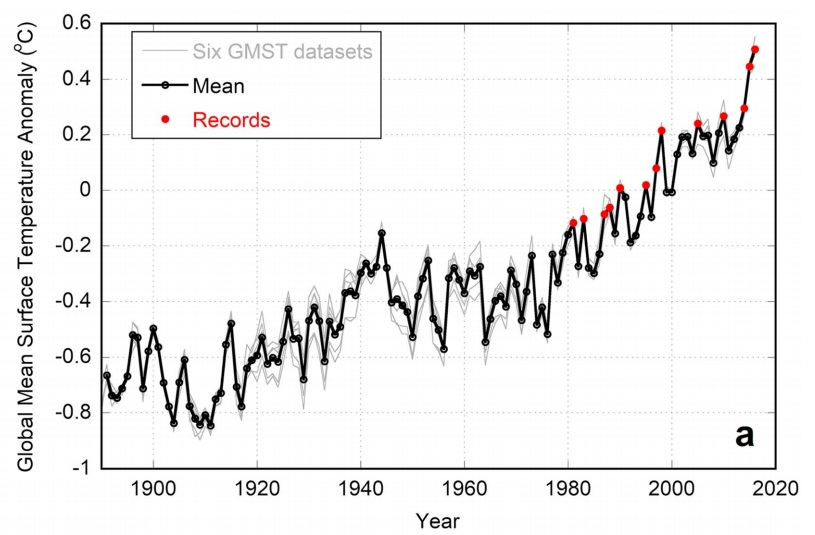
\includegraphics[scale=.6]{images/graphic.jpg}
			\caption{Gráfico representando o salto na temperatura global entre 1900 e 2020}
		\end{figure}

\end{document}